\chapter{Functional Abstraction}\label{ch:abstraction}

In \textbf{Intermediate Student with lambda}, functions are
\textbf{first-class values}: they can be passed as arguments, produced as
results, stored in lists and structures, and created without a name. This
lets us abstract the recurring recursive patterns into reusable
\textbf{higher-order functions}.

\section{Functions as arguments}
Compare two functions from Chapter 6:
\begin{lstlisting}[style=racket]
(define (keep-positive lon)
  (cond [(empty? lon) empty]
        [(positive? (first lon)) (cons (first lon) (keep-positive (rest lon)))]
        [else (keep-positive (rest lon))]))

(define (keep-even lon)
  (cond [(empty? lon) empty]
        [(even? (first lon)) (cons (first lon) (keep-even (rest lon)))]
        [else (keep-even (rest lon))]))
\end{lstlisting}
They differ only in the predicate. Make the predicate a parameter:

\begin{lstlisting}[style=racket]
;; (my-filter pred? lst) produces the elements of lst satisfying pred?.
;; my-filter: (X -> Bool) (listof X) -> (listof X)
(check-expect (my-filter even? '(1 2 3 4)) '(2 4))
(define (my-filter pred? lst)
  (cond [(empty? lst) empty]
        [(pred? (first lst)) (cons (first lst) (my-filter pred? (rest lst)))]
        [else (my-filter pred? (rest lst))]))
\end{lstlisting}

The contract uses a \textbf{type variable} \code{X}: \code{my-filter} works
for any element type, as long as the predicate consumes that type. Contracts
with type variables are called \textbf{generic} or \textbf{polymorphic}.

\section{lambda: anonymous functions}
Defining a named function just to pass it once is clumsy.
\code{(lambda (x1 ... xn) body)} produces a function value directly:
\begin{lstlisting}[style=racket]
(my-filter (lambda (n) (> n 10)) '(5 15 25))   ; => '(15 25)
((lambda (x y) (+ x (* 2 y))) 1 3)              ; => 7
\end{lstlisting}

In fact \code{(define (f x) body)} is shorthand for
\code{(define f (lambda (x) body))}. A function is just a value bound to a
name.

\begin{important}[Substitution rule for lambda]
\code{((lambda (x1 ... xn) exp) v1 ... vn)} $\Rightarrow$ \code{exp'} where
\code{exp'} is \code{exp} with each \code{xi} replaced by \code{vi}. A
\code{lambda} expression is itself a value.
\end{important}

\section{Functions as results}
\begin{lstlisting}[style=racket]
;; (make-adder n) produces a function that adds n to its argument.
;; make-adder: Num -> (Num -> Num)
(define (make-adder n)
  (lambda (x) (+ x n)))

(define add5 (make-adder 5))
(check-expect (add5 10) 15)
(check-expect ((make-adder 1) 1) 2)
\end{lstlisting}
Trace:
\begin{lstlisting}[style=racket]
((make-adder 1) 1)
=> ((lambda (x) (+ x 1)) 1)
=> (+ 1 1)
=> 2
\end{lstlisting}
The produced function ``remembers'' \code{n}; such a function together with the
bindings it captures is called a \textbf{closure}. Lexical scope determines
which \code{n} is meant. Combining \code{local} and \code{lambda} gives the same
effect with a named helper.

A closure can be pictured as the code of the \code{lambda} packaged with the
bindings it refers to:

\begin{center}
\begin{tikzpicture}[arr/.style={-{Stealth},thick}]
  \node[draw,rounded corners,fill=blue!6,font=\small\ttfamily] (call) at (0,0) {(make-adder 5)};
  \draw[rounded corners,fill=green!6] (2.9,-0.85) rectangle (9.4,0.85);
  \node[font=\scriptsize\bfseries,anchor=north west] at (2.9,0.85) {closure};
  \node[draw,fill=white,font=\small\ttfamily] (code) at (5.15,-0.2) {(lambda (x) (+ x n))};
  \node[draw,fill=white,font=\small\ttfamily] (env) at (8.45,-0.2) {n = 5};
  \draw[arr] (call) -- node[above,font=\scriptsize]{produces} (2.9,0);
  \node[font=\scriptsize\ttfamily,anchor=west] (nm) at (9.8,0) {add5};
  \draw[arr,gray] (nm) -- (9.4,0);
\end{tikzpicture}
\end{center}

\section{The built-in abstract list functions}

\begin{center}
\begin{tabular}{ll}
\toprule
Function & Contract \\
\midrule
\code{map} & \code{(X -> Y) (listof X) -> (listof Y)} \\
\code{filter} & \code{(X -> Bool) (listof X) -> (listof X)} \\
\code{foldr} & \code{(X Y -> Y) Y (listof X) -> Y} \\
\code{foldl} & \code{(X Y -> Y) Y (listof X) -> Y} \\
\code{build-list} & \code{Nat (Nat -> X) -> (listof X)} \\
\code{andmap}, \code{ormap} & \code{(X -> Bool) (listof X) -> Bool} \\
\code{apply} & \code{(X ... -> Y) (listof X) -> Y} \\
\bottomrule
\end{tabular}
\end{center}

\subsection{map}
\code{(map f (list x1 ... xn))} $=$ \code{(list (f x1) ... (f xn))}.
\begin{lstlisting}[style=racket]
(map sqr '(1 2 3))                         ; => '(1 4 9)
(map (lambda (s) (string-append s "!")) '("hi" "yo"))  ; => '("hi!" "yo!")
(map + '(1 2) '(10 20))                    ; => '(11 22)  (several lists)
\end{lstlisting}

\subsection{foldr}
\code{foldr} abstracts the ``combine'' pattern of structural recursion:
\[ \code{(foldr f base (list x1 x2 ... xn))} = \code{(f x1 (f x2 ... (f xn base)))} \]
\begin{lstlisting}[style=racket]
;; my-foldr: (X Y -> Y) Y (listof X) -> Y
(define (my-foldr combine base lst)
  (cond [(empty? lst) base]
        [else (combine (first lst) (my-foldr combine base (rest lst)))]))
\end{lstlisting}
The first argument of \code{combine} is the current element; the second is
the result of folding the rest. Many functions are one-liners:
\begin{lstlisting}[style=racket]
(define (sum lon) (foldr + 0 lon))
(define (count lst) (foldr (lambda (x rr) (add1 rr)) 0 lst))
(define (my-map f lst) (foldr (lambda (x rr) (cons (f x) rr)) empty lst))
(define (my-append l1 l2) (foldr cons l2 l1))
\end{lstlisting}
Trace:
\begin{lstlisting}[style=racket]
(foldr + 0 (list 1 2 3))
=> (+ 1 (foldr + 0 (list 2 3)))
=> (+ 1 (+ 2 (foldr + 0 (list 3))))
=> (+ 1 (+ 2 (+ 3 (foldr + 0 empty))))
=> (+ 1 (+ 2 (+ 3 0)))
=> 6
\end{lstlisting}

\subsection{foldl}
\code{foldl} abstracts the \emph{accumulator} pattern; it combines from the left:
\[ \code{(foldl f base (list x1 ... xn))} = \code{(f xn (... (f x2 (f x1 base))))} \]
\begin{lstlisting}[style=racket]
;; my-foldl: (X Y -> Y) Y (listof X) -> Y
(define (my-foldl combine acc lst)
  (cond [(empty? lst) acc]
        [else (my-foldl combine (combine (first lst) acc) (rest lst))]))

(define (my-reverse lst) (foldl cons empty lst))
(check-expect (my-reverse '(1 2 3)) '(3 2 1))
\end{lstlisting}

Drawn as trees, the two folds nest the applications of \code{f} in opposite
directions: \code{foldr} puts \code{base} next to the \emph{last} element,
\code{foldl} next to the \emph{first}.

\begin{center}
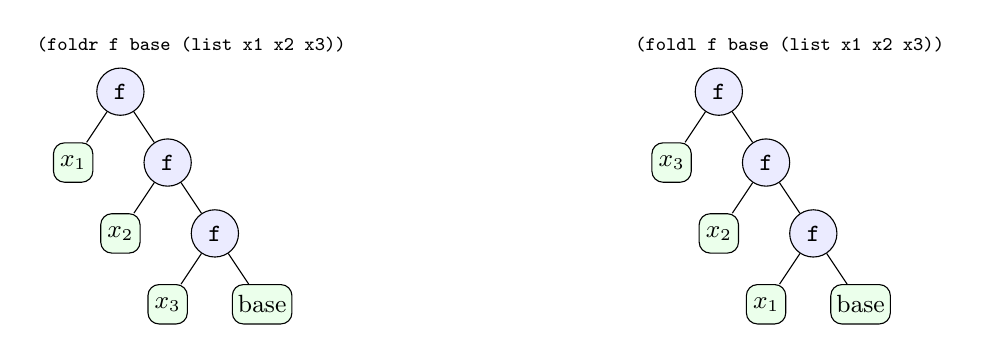
\begin{tikzpicture}[level distance=9mm,
  fn/.style={circle,draw,fill=blue!8,font=\ttfamily\small,minimum size=6mm,inner sep=0pt},
  lv/.style={draw,rounded corners,fill=green!8,font=\small,minimum size=5mm,inner sep=2pt},
  level/.style={sibling distance=12mm}]
  \node[fn] {f}
    child {node[lv] {$x_1$}}
    child {node[fn] {f}
      child {node[lv] {$x_2$}}
      child {node[fn] {f}
        child {node[lv] {$x_3$}}
        child {node[lv] {base}}}};
  \node[font=\scriptsize\ttfamily] at (0.9,0.6) {(foldr f base (list x1 x2 x3))};
  \begin{scope}[xshift=7.6cm]
  \node[fn] {f}
    child {node[lv] {$x_3$}}
    child {node[fn] {f}
      child {node[lv] {$x_2$}}
      child {node[fn] {f}
        child {node[lv] {$x_1$}}
        child {node[lv] {base}}}};
  \node[font=\scriptsize\ttfamily] at (0.9,0.6) {(foldl f base (list x1 x2 x3))};
  \end{scope}
\end{tikzpicture}
\end{center}

\subsection{build-list}
\code{(build-list n f)} $=$ \code{(list (f 0) (f 1) ... (f (sub1 n)))}; it abstracts recursion on \code{Nat}.
\begin{lstlisting}[style=racket]
(build-list 5 sqr)                   ; => '(0 1 4 9 16)
(define (countup-to n b) (build-list (add1 (- b n)) (lambda (i) (+ n i))))
\end{lstlisting}

\subsection{Combining abstractions}
\begin{lstlisting}[style=racket]
;; (sum-of-even-squares lon) produces the sum of squares of even
;;   elements of lon.
;; sum-of-even-squares: (listof Int) -> Int
(check-expect (sum-of-even-squares '(1 2 3 4)) 20)
(define (sum-of-even-squares lon)
  (foldr + 0 (map sqr (filter even? lon))))
\end{lstlisting}

Read from the inside out, the body is a pipeline:

\begin{center}
\begin{tikzpicture}[v/.style={draw,rounded corners,fill=green!8,font=\small\ttfamily,minimum height=6mm},
  arr/.style={-{Stealth},thick}]
  \node[v] (a) {'(1 2 3 4)};
  \node[v,right=23mm of a] (b) {'(2 4)};
  \node[v,right=23mm of b] (c) {'(4 16)};
  \node[v,right=23mm of c] (d) {20};
  \draw[arr] (a) -- node[above,font=\scriptsize\ttfamily]{filter even?} (b);
  \draw[arr] (b) -- node[above,font=\scriptsize\ttfamily]{map sqr} (c);
  \draw[arr] (c) -- node[above,font=\scriptsize\ttfamily]{foldr + 0} (d);
\end{tikzpicture}
\end{center}

\section{Abstraction with local and lambda}
Parameters of the enclosing function are visible inside a \code{lambda}:
\begin{lstlisting}[style=racket]
;; (scale-all k lon) multiplies each element of lon by k.
;; scale-all: Num (listof Num) -> (listof Num)
(define (scale-all k lon) (map (lambda (x) (* k x)) lon))

;; (above-avg lon) keeps the elements greater than the average.
;; above-avg: (ne-listof Num) -> (listof Num)
(define (above-avg lon)
  (local [(define avg (/ (foldr + 0 lon) (length lon)))]
    (filter (lambda (x) (> x avg)) lon)))
\end{lstlisting}

\section{Functional abstraction on other data}
Abstraction works for any recursive data. A generic fold over binary trees:
\begin{lstlisting}[style=racket]
;; bt-fold: (Num Y Y -> Y) Y BT -> Y
(define (bt-fold f base t)
  (cond [(empty? t) base]
        [else (f (node-key t)
                 (bt-fold f base (node-left t))
                 (bt-fold f base (node-right t)))]))

(define (size t) (bt-fold (lambda (k l r) (+ 1 l r)) 0 t))
(define (tree-sum t) (bt-fold (lambda (k l r) (+ k l r)) 0 t))
\end{lstlisting}

\section{When to use what}
\begin{itemize}
  \item Each element transformed independently $\to$ \code{map}.
  \item Keep some elements $\to$ \code{filter}.
  \item Combine all elements into one value $\to$ \code{foldr} (or \code{foldl} for accumulator-style).
  \item Generate a list from indices $0..n-1$ $\to$ \code{build-list}.
  \item Test whether all/any satisfy a predicate $\to$ \code{andmap}/\code{ormap}.
  \item Processing that needs early stopping, two lists at different rates, or generative recursion usually needs explicit recursion.
\end{itemize}

\section{Contracts for higher-order functions}
\begin{itemize}
  \item Function types are written in parentheses: \code{(Num -> Bool)}.
  \item Use type variables (\code{X}, \code{Y}) when the function is generic; the same variable must stand for the same type throughout a contract.
  \item Example: \code{compose: (Y -> Z) (X -> Y) -> (X -> Z)}.
\end{itemize}

\section{Summary}
\begin{itemize}
  \item Functions are first-class values; \code{lambda} creates them anonymously.
  \item Abstracting a common pattern means turning the differing part into a function parameter.
  \item \code{map}, \code{filter}, \code{foldr}, \code{foldl}, \code{build-list} capture the main list recursion patterns.
  \item A function produced by another function captures the bindings it refers to (closure).
  \item Generic contracts use type variables.
\end{itemize}
